\chapter{Claim Structuring}
\label{chap:claim_structuring}

In the previous chapter, we have introduced two approaches to formalize 
claims.  Having formalized claims can help in inferring claims
or help with related downstream tasks (such as stance classification) as it
will be shown in chapter~\ref{chap:analysis}.
Formalized claims can be obtained manually, applying the steps laid out in the 
claim ontology framework in chapter~\ref{chap:formalization}. 
In this chapter, we wish to explore how some of the steps of the ClaimOntology
framework can be automatized. 
In particular, we focus on formalizing 
claims, assuming that the rest of the framework is already setup. 
Thus, we work in a setting where the domain ontology has been determined (domain is
restricted and closed) we wish to explore how feasible it is to automatically
acquire formalized claims from raw text claims: solve the \textbf{claim structuring}
problem.

First, we explain how we adopt the dataset which will be used for claim
structuring in section~\ref{sec:claim_struc_data}.  Then we define models that
attempt to solve the claim structuring problem in
section~\ref{sec:claim_struc_models}.  The models are evaluated across multiple
setups in section~\ref{sec:claim_struc_experiment}.  

\section{Data}
\label{sec:claim_struc_data}

We use the ontology formalizations from the 
``\emph{Marijuana}'' topic built in section~\ref{sec:usecase_ontology} and 
want to see how feasible it is to obtain them automatically from raw text.
We focus on claim individual formalizations which we obtain by exporting
the integrated upper and domain ontology populated with claim individuals. 
The ontology contains a total of 920 claims. Out of those 920, three annotators 
A1, A2, and A3 manage to formalize 864, 867, and 860 claims respectively.
We take formalizations from annotator A1. 
Next, we attempt to formulate claim structuring as a supervised learning
problem.  Two basic approaches are considered: predicting components of the
formalization then putting them together (binary relevance, \texttt{BR}), or
predicting the entire formalization (label powerset, \texttt{LP}). 
Using components corresponds to a more realistic scenario, as it reflects 
the process of manually building a claim formalization. 

Following the \texttt{BR} approach, a formalized ontology claim can be broken
down into four components:
\begin{itemize}
	% TODO add mathematical notation from ontology section
	\item \emph{modality} ($\mathit{MOD} \in \{\mathit{fact},
		\mathit{good\_value}, \mathit{bad\_value}, \mathit{policy}\}$), 
	\item \emph{count} ($\mathit{CNT} \in \{\mathit{unary},
		\mathit{binary},  \mathit{ternary}\}$),
	\item \emph{properties} ($\mathit{PR} \in \{\mathit{has\_antecedent},
		\mathit{has\_declaration}, \mathit{implies}, \dots\}$)
	\item \emph{domain individuals} ($\mathit{DI} \in \{\mathit{marijuana},
		\mathit{legalized\_marijuana}, \mathit{mafia\_bankrupt},
		\dots\}$)
\end{itemize}
The \emph{count} component reflects how many object properties the claim individual
contains (a claim with a $\mathit{has\_declaration}$ property has $\mathit{unary}$ count, etc.).
Now, to construct a formalized claim, we use a exactly one (out of four
possible) \emph{modality}, exactly one (out of three possible) \emph{count},
one or more (up to three, out of 22 possible) \emph{properties}, and one
or more (out of 82 possible) \emph{domain individuals} (one for each property). 
We could have had negation as an extra component of the formalized claim, but
since only properties may be negated, we construct the properties set $PR$ as a
union of properties and their respective negations: 
$$
P = \{\mathit{has\_antecedent}, 
\mathit{negated\_has\_antecedent}, \mathit{implies}, \mathit{not\_implies}\, \dots\}
$$

Taking into consideration all possible combinations of components from
annotator A1, 107 binary labels ($82 \cdot \mathit{DI} + 17 \cdot \mathit{PR} + 4\cdot
\mathit{CNT} + 7 \cdot \mathit{MOD}$) can be assigned to a claim, from which a
formalized claim can be constructed.  This means that there  exists an
exponential ($2^{107}$) number of possible formalizations, a large number of
which is invalid.  An invalid formalization example would involve both the
\texttt{has\_declaration} and \texttt{has\_antecedent} property which is not allowed,
since \texttt{has\_declaration} can only be assigned to a \texttt{unary} claim,
whereas \texttt{has\_antecedent} can only be assigned to \texttt{binary} claim. 

\begin{figure}
	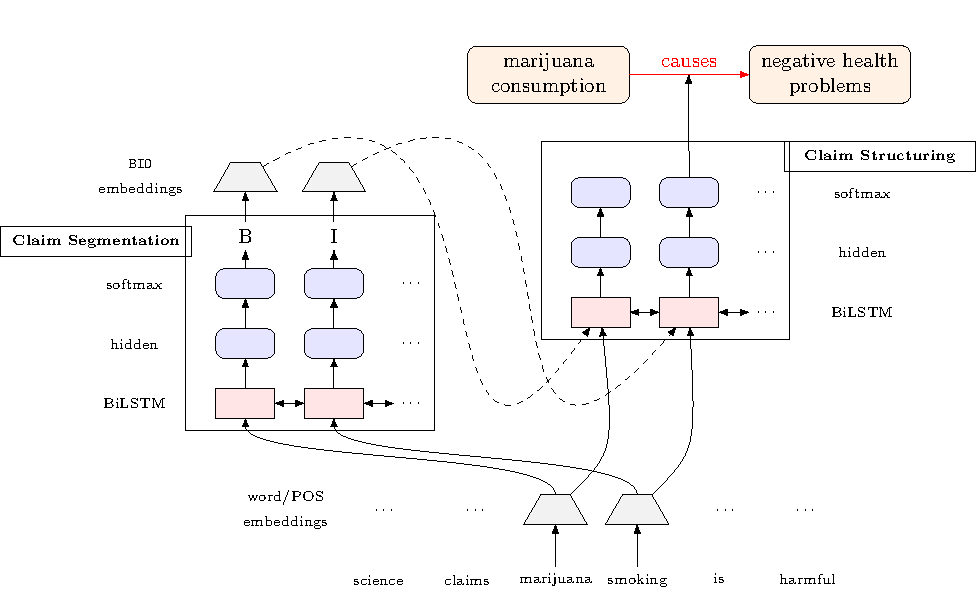
\includegraphics{joint_tikz-figure0.pdf}
	\caption{Joint BiLSTM model for both claim segmentation and claim 
	structuring. }
	\label{fig:joint_model}
\end{figure}

\section{Models}
\label{sec:claim_struc_models}

We wish to build models for claim structuring. The models should produce 
formalized claims from text. 
Three model setups are proposed: independent classifiers, 
chain classification, and a joint model. 

\paragraph{Independent classifiers (IND). }
As a baseline approach, we use independent SVMs to predict formalization
components.
For SVM features, we use distributed word representations
(fastText\footnote{https://fasttext.cc/}
and word2vec\footnote{https://code.google.com/archive/p/word2vec/}
pretrained vectors).
To train each independent model, we use $5 \times 3$ nested-cross validation
and optimize hyperparameters $C$ and $\gamma$ using grid search. 
We experiment with both the \texttt{BR} and \texttt{LP} approach.

% gold labels in predictions
% lab_id     1.000000
% iternum    2.000000
% foldnum    2.000000
% prec       0.930443
% recall     0.777855
% f1         0.817828
% dtype: float64
% 11
% lab_id     8.000000
% iternum    2.000000
% foldnum    2.000000
% prec       0.706546
% recall     0.698467
% f1         0.698874
% dtype: float64
% 82
% lab_id     47.609489
% iternum     1.751825
% foldnum     1.751825
% prec        0.100942
% recall      0.060585
% f1          0.069552
% dtype: float64
% 4
% lab_id     97.500000
% iternum     2.000000
% foldnum     2.000000
% prec        0.689005
% recall      0.700169
% f1          0.691263
% dtype: float64
% lab_id     42.445055
% iternum     1.813187
% foldnum     1.813187
% prec        0.258942
% recall      0.221668
% f1          0.229637

\paragraph{Chain classification (CC). }
To take advantage of formalization component dependencies, we adopt the chain
classification approach, as described in
section~\ref{sec:chain_classification}.
First, to verify the label dependency assumption we build a chain classifier
which uses gold  labels as input in each prediction.  
This yields performances an overall performance of average of $0.23$ F1-score. 
The domain properties prove the hardest to predict, as removing them yields
an average of $0.71$ F1-score. 
This promising performance is more than enough reason to adopt the
chain classification approach for claim formalization. 
We frame all component classifications as either multiclass or multi-label classification.
We prefer to use multiclass classification where possible 
(count and modality component prediction), since
generalizing multiclass to multi-label classification likely degrades performance
due to loss of information between classes. 
SVMs models are then chained such that the prediction of one SVM is added as
input to the following SVM model, until all labels are predicted. 
We randomize the ordering of labels which are predicted.
Additionally, to alleviate the influence of randomization, we 
ensemble chain classifiers (ECC) using a majority vote. 
To train the model, we use $5 \times 3$ nested-cross validation
and optimize hyperparameters $C$ and $\gamma$ using grid search. 
It is sensible to use the chain classification model only in the
\texttt{BR} setup.

\paragraph{Joint model (BiLSTM-J). } 
Apart from dependencies in the claim structure, we wish to investigate whether
it is feasible to derive the claim structure directly from text. 
To that end, we present a joint model which does claim segmentation (details described in
chapter~\ref{chap:claim_structuring}) and claim structuring in one step. We
draw inspiration from \citep{miwa2016end} where they use consecutive
LSTM cells to predict multiple outputs. We adopt a similar approach, where we
use two sets of BiLSTM layers: first (\texttt{BiLSTM-seg}), to predict claims, and
second (\texttt{BiLSTM-struc}) to perform claim formalization of the predicted claims. The
\texttt{BiLSTM-seg} layer is a shared, as we wish to update its parameters
when upon incorrect formalization in addition to incorrect claim segmentation.

The input of the \texttt{BiLSTM-seg} layer is a sequence of tokens and their
respective part-of-speech (POS) tags \citep{brown1957linguistic} paired \texttt{BIO}
tags (explained in section~\ref{sec:claim_seg_problem}). 
The \textit{BiLSTM-seg} layer produces \texttt{BIO} tags, which are then converted to textual
claims. Then, in the \textit{BiLSTM-struc} part, component classifiers
are hooked to the predicted input claim text. Component classifiers
consist of a BiLSTM and a linear layer. Softmax is applied to 
the multiclass modality and count classifiers, whereas the sigmoid function is
applied to the multi-label to the domain individual and property classifiers in
order to obtain label probabilities. 
The output of the \textit{BiLSTM-struc} are class probabilities for all four 
formalized claim components. 
The model architecture is illustrated in Fig.~\ref{fig:joint_model}. 
We use three sets of embeddings: word, POS embeddings, and \texttt{BIO} tag
embeddings. We optimize using the stochastic gradient descent algorithm
with a learning rate of $0.01$ and use L2 penalty for regularization. 
Negative log-likelihood loss is used to calculate loss for
\texttt{BIO} tags, formalization modality, and formalization count.
Binary cross-entropy is used to calculate loss for formalization
properties and formalization domain individuals, since they are used in a 
multi-label setup). 
The loss of the joint model is simply a sum of all individual losses. 
We experiment with and without pretrained word embeddings. 
The joint model is applied for both the \texttt{BR} and 
\texttt{LP} setup. 

\section{Experiments}
\label{sec:claim_struc_experiment}

\begin{table}
	\centering
\renewcommand{\arraystretch}{2}%
	\begin{tabular}{p{3cm} c c c c  c  c c c  @{\hspace{1.5em}}c@{}  @{\hspace{1em}}c@{}  }
	\toprule
		\multirow{2}{*}{Model / Setup}
		& \multicolumn{2}{c}{\texttt{MOD}} 
		& \multicolumn{2}{c}{\texttt{CNT}} 
		& \multicolumn{2}{c}{\texttt{PR}}
		& \multicolumn{2}{c}{\texttt{DI}} 
		& \multicolumn{2}{c}{\texttt{CL}}
		\\

		& OR  & PA  & OR  & PA  & OR  & PA & OR  & PA &  OR & PA \\
		\midrule

		RAND & \multicolumn{2}{c}{0.25} & \multicolumn{2}{c}{0.32} & \multicolumn{2}{c}{0.10} & \multicolumn{2}{c}{0.04} & \multicolumn{2}{c}{0.00} \\
		IND & \textbf{0.84} & 0.90 & \textbf{0.79} & \textbf{0.87} & 0.11 & 0.24 & \textbf{0.05} & 0.13 & 0.00 & 0.00  \\		
		CC & \textbf{0.84} & \textbf{0.91} & \textbf{0.79} & \textbf{0.87} & 0.14 & 0.39 & 0.03 & 0.05 & 0.02 & 0.03 \\
		ECC & 0.80 & 0.88 & 0.77 & \textbf{0.87} & \textbf{0.15} & \textbf{0.41} & 0.04 & \textbf{0.06} & \textbf{0.03} & \textbf{0.04} \\
		BiLSTM-J & 0.52 & / &  0.33 & / & 0.11 & / &  0.00 & / & 0.00 & / \\

		\bottomrule
	\end{tabular}
	\caption{
	Macro-averaged F1-score comparison between 
	the independent SVM (IND), randomized classifier (RAND), chain classification (CC), 
	ensemble chain classification (ECC), and joint model (BiLSTM-J)
	in the task of 
	claim structuring from both original (OR) and paraphrased text claims (PA)
	using the \texttt{BR} approach. 
	Results are compared on individual components
	across modalities (\texttt{MOD}), counts (\texttt{CNT}), 
	properties (\texttt{PR}), and 
	domain individuals (\texttt{DI}). Finally, predictions are assembled into a 
	formalized claim and compared against the gold formalized claims (\texttt{CL}).
	Best results for each setup are boldfaced.
	}
	\label{tab:claim_struc_per_component}
\end{table}

% reltypes_binary, relation_matrix, property_matrix, fvp_binary), axis=1
% ranges_tutta = [reltypenum, relnum, propnum, fvp_num]

We perform two sets of experiments. First, we wish to explore models
that predict the formalization structure on a per-component basis (\texttt{BR}). 
Second, we investigate how does per-component prediction (\texttt{BR}) compares to 
the label powerset (\texttt{LP}) approach.
We execute all experiments using original and paraphrased claims, since we're
also interested in the practical uses of claim paraphrases.

\paragraph{Claim structuring feasibility. }
We attempt to predict the claim formalization in the binary
relevance (\texttt{BR}) setup to see how feasible is the claim 
structuring task. We use the \texttt{BR} since we believe it corresponds
to a more realistic scenario, particularly in the scenario where the number
of properties or domain individuals grows. In that scenario, using the
label powerset approach, we can expect that the
distribution of observed formalizations is long tailed, therefore it is not
feasible to expect to correctly predict infrequently seen formalizations.
Table~\ref{tab:claim_struc_per_component} shows macro averaged F1-scores for
the randomized classifiers (RAND), independent SVM classifiers (IND), chain
classifiers (CC), ensemble chain classifiers (ECC), and the joint segmentation
and structuring BiLSTM model (BiLSTM-J). We experiment with both original
source claims $OR$ (as they were written by the authors) and paraphrased claims $PA$ (as
they were transcribed by annotators).
Models are trained to predict components, with their predictions then assembled
together to constitute a formalized claim, which is compared against the gold
formalized claim.  The baseline is set using the randomized 
class for all individual components. The randomized baseline does not work 
based on input, therefore has the same results for both the $OR$ and $PA$ setup. 
The joint model might not produce the same number claim formalizations, 
so we evaluate on a comment level and average across all comments. Further, the joint
model can not use paraphrased claims since it works with the unsegmented comment. 
Additionally, we could have regularized the models by preventing invalid
formalizations perhaps in the form of constraint programming, but leave this
for future work. 

Overall, recognizing the entire formalized claim looks like an extremely
challenging task, since the best performing model ($ECC$) manages to achieve
only $0.03$ and $0.04$ macro-averaged F1-score
using original and paraphrased claims, respectively. This is mainly due
to the low performance of recognizing domain individuals in a claim.
Recognizing domain individuals in a claim is expectedly difficult, since there
are 75 sparsely distributed domain individuals, and only 847 claims.
Inspecting the component outputs of the indenpedent classifier, we conclude
that it mostly manages to correctly classify up to two components (mostly $MOD$
and $CNT$), but never manages to identify three or all four
components correctly, hence it never outputs the correct claim formalization. 
Unlike the $IND$ setup, the $CC$ and $ECC$ models managed to produce fully
accurate formalizations, and correctly predict three out of four component parts
in roughly 25\% of cases.
Even though the $CC$ and $ECC$ models exhibit performance drops in recognizing
$MOD$ and $CNT$ compared to individual classifiers, overall they seem like the most
promising options to formalize claims. 

%  final BIO                                                                                                                                                                                                    
%  ####################                                                                                                                                                                                         
%  precision basic 188 573 0.32809773123909247                                                                                                                                                                  
%  recall basic 188 631 0.2979397781299525                                                                                                                                                                      
%  offset 394 573 0.68760907504363                                                                                                                                                                              
%  offset 394 631 0.624405705229794                                                                                                                                                                             
%  ####################                                                                                                                                                                                         
%  final reltype                                                                                                                                                                                                
%  ####################                                                                                                                                                                                         
%  /home/filip/Documents/Doktorski/argontology/src/env/lib/python3.6/site-packages/sklearn/metrics/classification.py:1437: UndefinedMetricWarning: Precision and F-score are ill-defined and being set to 0.0 in
%    'precision', 'predicted', average, warn_for)                                                                                                                                                               
%    (array([0.        , 0.56118881, 0.9543877 ]), array([0.        , 0.70549451, 0.96855346]), array([0.        , 0.62512171, 0.9614184 ]), array([ 176,  455, 3975]))                                         
%    (0.5051921719001541, 0.5580159882046675, 0.5288467060081589, None)                                                                                                                                         
%    ####################                                                                                                                                                                                       
%    final fvp                                                                                                                                                                                                  
%    ####################                                                                                                                                                                                       
%    (array([0.58041958, 0.        , 0.        , 0.        , 0.9543877 ]), array([0.71397849, 0.        , 0.        , 0.        , 0.96855346]), array([0.64030858, 0.        , 0.        , 0.        , 0.9614184
%    (0.3069614569862463, 0.3365063907486306, 0.3203453973489082, None)                                                                                                                                         
%    ####################                                                                                                                                                                                       
%    final relation                                                                                                                                                                                             
%    ####################                                                                                                                                                                                       
%    /home/filip/Documents/Doktorski/argontology/src/env/lib/python3.6/site-packages/sklearn/metrics/classification.py:1437: UndefinedMetricWarning: Precision and F-score are ill-defined and being set to 0.0 
%      'precision', 'predicted', average, warn_for)                                                                                                                                                             
%      relation avg f1: 0.03323903818953324                                                                                                                                                                     

% joint model analysis
The joint \textit{BiLSTM-J} model performs worse than the $IND$, $CC$, and $ECC$
models, but better than the random baseline in three out of four categories.
This indicates that jointly extracting claims and structuring claims is an
extremely difficult task. The joint model fails to successfully extract and
formalize a single claim. 
The performance of the joint model in claim segmentation is slighly better than the 
$SVM$ model in section~\ref{sec:claim_seg_experiment} outperforming it by 
$0.07$ and $0.06$ macro-averaged F1-score percentage points. However, this still means
that the \textit{BiLSTM-struc} part of the joint model uses incorrect claim segments
a large portion of the time. 
Our suspicion that this might be causing poor performance is confirmed upon
seeing the joint model outputs, as we notice that the formalization predictions
are particularly bad when predicted claims are far from sensible. 

In an attempt to improve the joint model, we experiment with setting lower
learning rates for the shared \textit{BiLSTM-seg} layer, but to no significant
performance boost.  We then inspect the biggest contributers to the loss during
model training.  The highest contributor, by far, is the loss caused by $DI$
prediction.  We then manually try to assign weights to loss functions to
prevent a single component prediction from dominanting the total loss score.
By weighting the loss, we do obtain slightly better performance, but consider
this to be a solely short-term workaround. 
Additionally, we may try to train this model in using soft parameter sharing
 where the distance between the parameters of the
model is regularized to encourage model parameters to be similar
\citep{ruder2017overview}.

% \begin{table}
% 	\centering
% \renewcommand{\arraystretch}{2}%
% 	\begin{tabular}{p{3cm} c c }
% 	\toprule
% 		\multirow{2}{*}{Model / Setup}
% 		& \multicolumn{2}{c}{\texttt{LP}}
% 		\\
% 		& OR  & PA \\
% 		\midrule
% 		\textit{IND} &  0.08 & 0.14 \\		
% 		\textit{BiLSTM-J} & & \\
% 		\bottomrule
% 	\end{tabular}
% 	\caption{Claim structuring
% 	macro-averaged F1-score using the 
% 	binary relevance (\texttt{BR}) 
% 	and label powerset (\texttt{LP}) 
% 	approach for original (OR) and paraphrased (PA) claims. 
% 	}
% 	\label{tab:claim_struc_atomic_molecular}
% \end{table}

\paragraph{Predicting components \texttt{BR} or entire formalizations \texttt{LP}.} 
Even though the
\texttt{BR} approach is the more realistic setup, we now compare it
to the \texttt{LP} setup. For the \texttt{LP} setup
we map each claim formalization to a label and employ a single multiclass
classifier to predict the claim formalization from the claim text.
To obtain \texttt{LP} classes, first we generate all possible combinations of 
formalization components yielding $23\,318\,832$ possible combinations.
Then we restrict the space of possible solutions to only feasible ones
resulting in the final $10\,652\,784$ classes, but only 384 classes
occur in the dataset used. 
We omit results from both the majority and random classifers since they
perform extremely poorly ($<0.01$ macro-averaged F1-score).
% Results are listed in table~\ref{tab:claim_struc_atomic_molecular}.
We employ the $IND$ and \texttt{BiLSTM-J} model. The IND model achieves 
$0.08$ and $0.14$ macro-averaged F1-score using original and
paraphrased claims, respectively. This is significantly higher than 
$IND$ model in the \texttt{BR} setup where the model achieved less than $0.01$
macro-averaged F1-score percentage points in using both original and paraphrased claims.
As for the \texttt{BiLSTM-J} model, it achieves similarly poor results as in the
\texttt{BR} setup -- no more than $0.01$ macro-averaged F1-score. 
We conclude that using the \texttt{LP} setup gives better results than the 
\texttt{BR} setup. However, due to the size of the dataset and number of potential 
classes, we expect that model performance using the \texttt{LP} frame
will degrade in a larger and more diverse dataset. 

% 279 # weighted 0.270870342083376                                                                                                                                                                                   
% 280 # macro 0.14793585458242742                                                                                                                                                                                    
% 281 # micro 0.3047225264695144                                                                                                                                                                                     
% 282 #                                                                                                                                                                                                              
% 283 # ORIG                                                                                                                                                                                                         
% 284 # avg_score(scores_expansion_orig)                                                                                                                                                                             
% 285 # weighted 0.15657690759197077                                                                                                                                                                                 
% 286 # macro 0.08455041836472887                                                                                                                                                                                    
% 287 # micro 0.18802847754654986                                                                                                                                                                                    

All experiments clearly show that using paraphrases proved useful for
\textbf{all} approaches.  The models that use paraphrases outperform models
using original claims by an average of $0.08$ macro-averaged F1-score
percentage points.  This clearly suggests that having claim paraphrases is not
only useful for annotators when formalizing claims, but also for machine
learning algorithms doing claim structuring.  We hypothesize this is mostly due
to the reduction of noisiness and vagueness of claims.  In subsequent work, we wish
to further research the advantages of claim paraphrases, in addition to 
exploring deriving paraphrased, denoised claims from original ones. 

After we have explored the feasibility of automatic claim structuring, in the
next chapter we will explore the benefits of having formalized claims. 
We demonstrate examples of argumentation analysis one can perform using
formalized claims. 

% TODO some conclusion on the joint model vs. no joint model

% \section{Conclusion}
% \label{sec:claim_struc_conclusion}
% 
% In this chapter, we experimented with claim structuring. 
% We used the ontology formalizations are adapted them for 
% machine learning models in a binary relevance and label powerset setup. 
% We evaluate multiple models, some of them using structured prediction to obtain 
% results of \todo{add results}. From the results, it is 
% visible that \todo{add what is visible}
% We conclude that claim structuring is in general a difficult problem to solve,
% but with the help of structured approaches can achieve decent. 
% \todo{write more in the conclusion}
% %TODO give some decent number .
% Interestingly to note, results using paraphrased claims are significantly
% better across all models on average by F1-score points, which shows claim
% paraphrases make it easier to process claims for both humans and machines (each
% in their own way). 
% % TODO use paraphrased number - original average across all 
